\section{IP mapping}
L'ultimo problema che viene descritto  è stato anche il
più difficile da risolvere, e che, potenzialmente, avrebbe potuto far fallire
tutto il lavoro precedentemente fatto.

\subsection{Il problema}
Si è detto in precedenza che si è scelta infine una configurazione \textit{Local
Server}, con i server OpenVPN installati in MoonCloud e raggiungibili mediante IP
pubblici dai client presenti nella rete target. Per ragioni di costi, si vuole
limitare il numero di VM in MoonCloud con OpenVPN in esecuzione, e quindi poter
dedicare un singolo server a servire più reti target contemporaneamente. OpenVPN
consente di isolare i singoli client connessi ad un server, infatti di default
tali client possono comunicare solo con il server, e non con altri client (a meno
che si utilizzi la direttiva ``\texttt{client-to-client}'').\\
Per poter realizzare in maniera corretta una topologia del genere è
\textit{fondamentale che ogni rete target abbia un spazio di indirizzamento diverso} \cite{openvpn-lan-to-lan}.
Tuttavia qui sorge il problema: ciascuna LAN target ragionevolmente usa uno o più
pool di indirizzi privati, i quali sono limitati. In \cite{RFC1918} si
stabilisce che i seguenti spazi di indirizzi siano riservati per l'utilizzo esclusivo
in una rete privata e che non siano instradabili su Internet:
\begin{itemize}
	\item classe A (subnet mask a 8 byte) \texttt{10.0.0.0} -- \texttt{10.255.255.255}
	\item classe B (subnet mask a 16 byte) \texttt{172.16.0.0} -- \texttt{172.31.255.255}
	\item classe C (subnet mask a 24 byte) \texttt{192.168.0.0} -- \texttt{192.168.255.255}
\end{itemize}
Può accadere che tali indirizzi siano utilizzati con una subnet mask diversa, ad esempio
\texttt{10.1.1.0/24}. Rimane
comunque il fatto che i detti prefissi sono tipicamente quelli che si trovano
in una qualsiasi LAN con IPv4.\\
E' chiaro che la probabilità che diverse reti target abbiano lo stesso NET ID
è alta, diventa
quindi un grosso problema poter collegare più
reti target ad uno stesso VPN server, proprio a causa della possibilità che prima o poi
si verifichi un conflitto.\\
Stabilire a priori un mappaggio tra VPN server e reti clienti (es: si definisce
il server \texttt{OpenVPN\_1--20} che gestirà reti \texttt{10.0.0.0/24 -- 10.20.20.0/24})
non risolve il problema: cosa fare se ad un certo punto ci si trova con due clienti con
entrambi \texttt{10.1.1.0/24}?\\
Un'altra soluzione potrebbe essere quella di allocare un server OpenVPN
per ogni cliente. Lato MoonCloud si creano $n$ Exection Cluster, uno per ciascun cliente,
costituiti da un VPN server e almeno da un \textit{Docker host}. Ciascun cluster è isolato,
quindi i conflitti non hanno nessun impatto. Si è deciso di lasciare questa strada per ultima,
perché per quanto funzioni presenta un grosso incoveniente: farebbe aumentare di molti i
costi. Più il numero di client aumenterebbe maggiore sarebbe il numero di VM per OpenVPN server
da allocare, tanto più i costi salirebbero.\\
Ecco quindi il problema che si è dovuto risolvere: \textit{come gestire
	la conflittualità tra gli indirizzi IP delle reti target senza dover allocare un
server OpenVPN per ogni cliente?}


\subsection{La soluzione}
L'idea alla base della soluzione è quella di \textit{mappare} ogni rete target
su una nuova rete, stabilita da MoonCloud e garantita univoca.
``\textit{Mappare}'' una rete significa trovare una nuovo NET ID per tale rete, e
\textit{spostare} gli indirizzi IP originali nel nuovo NET ID. Lato MoonCloud, i
\textit{probe} conoscono gli indirizzi IP modificati (garantiti univoci), ed il rimappaggio
verso quelli originali viene effettuato sul device VPN client.\\
Prima di proseguire, si chiarisce meglio la terminologia che da qui in poi sarà utilizzata:
\begin{itemize}
	\item ``\textit{rete originale -- OTN (Original Target Network)}'': l'indirizzo IP di rete della rete target così come
	      è in realtà
	\item ``\textit{IP originale -- OTI (Original Target IP)}'': l'indirizzo IP di un
	      host nella rete target così
	      come è in realtà
	\item ``\textit{rete mappata -- MTN (Mapped Target Network)}'': il nuovo NET ID
	      assegnato ad una rete target
	\item ``\textit{IP mappato -- MTI (Mapped Target IP)}'': l'indirizzo IP appartenente alla \textit{rete
		mappata} a cui corrisponde un indirizzo IP originale
		\item ``\textit{rete rimappata -- RTN (Remapped Target Network)}'':  l'indirizzo
		      IP di rete della rete target così
		      come è in realtà, ovvero uguale alla \textit{rete originale}
		\item ``\textit{IP rimappato -- RTI (Remapped Target IP)}'': corrisponde all'\textit{IP originale}.
		\item ``\textit{mappare una rete}'': assegnare alla \textit{rete originale} una
		      \textit{rete mappata}
		\item ``\textit{mappare un indirizzo IP}'': assegnare un \textit{IP mappato}
		      ad un \textit{IP originale}
		\item ``\textit{rimappare una rete}'': procedimento inverso del
		      ``\textit{mappare una rete}''
		\item ``\textit{rimappare un indirizzo IP}'': procedimento inverso del
		      ``\textit{mappare un indirizzo IP}''
		      % \item ``\textit{SMTN (Set of Mappped Target Networks)}'': l'insieme di reti mappate
	\end{itemize}
	Si definiscono quindi
	le seguenti funzioni \textit{deterministiche} (con $S$ corrispondente ad un certo
	server OpenVPN):
	\begin{itemize}
		\item $map\_network: OTN, S \rightarrow MTN$, una funzione cha data una
		      $OTN$ ritorna una $MTN$, garantita univoca per il server $S$
		\item $map\_address: OTI, OTN, MTN, S \rightarrow MTI$,
		      una funzione che dato in input:
		      \begin{itemize}
		      	\item $OTI \mid OTI \in OTN$: un indirizzo IP originale appartenente alla
		      	      rete originale
		      	\item $OTN$: la rete originale
		      	\item $MTN \mid map\_network(OTN)=MTN$: la rete mappata della rete originale
		      	\item $S$: il server OpenVPN a cui $OTN$ è assegnata
		      \end{itemize}
		      ritorni $MTI$: un indirizzo $\in MTN$ corrispondente a $OTI$.
		\item $remap\_network: MTN, S \rightarrow OTN$, una funzione che data una rete
		      mappata ritorna la corrispondente rete originale assegnata ad un certo server,
		      con $OTN=RTN$.
		\item $remap\_address: MTI, MTN, OTN, S \rightarrow OTI$, una funzione che dato
		      in input:
		      \begin{itemize}
		      	\item $MTI \in MTN$: indirizzo IP mappato
		      	\item $MTN \mid map\_network(OTN)=MTN$: la rete $OTN$ mappata
		      	\item $OTN$: la rete originale
		      	\item $S$  il server OpenVPN a cui $OTN$ è assegnata
		      \end{itemize}
		      ritorna $OTI$: un indirizzo $\in OTN$ corrispondente a $MTN$, e $RTI=OTI$
	\end{itemize}
	Per queste funzioni valgono le seguenti uguaglianze:
	\begin{itemize}
		\item $remap\_network(map\_netowrk(OTN, S), S)=map\_network(OTN, S)^{-1}$
		\item
		      $remap\_address(map\_address(OTN, OTI, MTN, S), MTN, OTN, S)=\\
		      map\_address(OTN, OTI, MTN, S)^{-1}$
	\end{itemize}
	In altre parole, ogni funzione è l'inverso dell'altra.\\
	\textit{Come effettuare il mappaggio?}
	La funzione $map\_network$ deve essere per forza di cose effettuata dai VPN client,
	in modo che i server ``vedano'' sempre reti univoche. Non solo, questa tecnica di mapping deve
	rispettare ed integrarsi alla perfezione con il \textit{NAT al contrario}, il cui
	utilizzo è imprescindibile.
	La soluzione implementativa è anche in questo caso iptables. 
		
	Si supponga di avere la seguente configurazione:
	\begin{itemize}
		\item rete target $OTN$: \texttt{192.168.100.0/24}
		\item \texttt{CommonName} VPN client: \texttt{client1}
		\item rete mappata: $map\_network(OTN, S)=$\texttt{192.168.1.0./24}
		\item rete MoonCloud: \texttt{192.168.200.0/24}
		\item indirizzo IP interno VPN server $S$: \texttt{192.168.200.20}
		\item indirizzo IP pubblico VPN server: \texttt{100.4.78.5}
		\item indirizzo IP del \textit{Docker host}: \texttt{192.168.200.2}
		\item indirizzo IP VPN client ($OTI \in OTN$): \texttt{192.168.100.50}
		\item subnet VPN: \texttt{10.7.0.0/24}
		\item indirizzo IP scheda di rete virtuale VPN server: \texttt{10.7.0.1}
		\item indirizzo IP scheda di rete virtuale VPN client: \texttt{10.7.0.2}
		\item \texttt{CommonName} del VPN client: \texttt{client1}
		\item target da analizzare ($OTI \in OTN$): \texttt{192.168.1.254}
		\item target mappato: $MTI \in MTN=map\_address(\texttt{192.168.100.254},\\
		      \texttt{192.168.100.0/24},
		      \texttt{192.168.1.0/24})=\texttt{192.168.1.254}$
	\end{itemize}
		
		
	% Quando il VPN client riceve dei pacchetti dalla NIC virtuale di OpenVPN iptables
	% esegue le seguenti operazioni:
	% \begin{enumerate}
	%   \item modificare l'indirizzo
	%   IP destinazione dei pacchetti appena sono stati ricevuti dalla VPN
	%   (applicando la funzione $remap\_address$), in modo che abbiano per destinazione quello reale
	%   \item applicare il \textit{NAT al contario} per modificare l'indirizzi IP sorgente
	% \end{enumerate}
	% Quando si ricevono dei pacchetti risposte a richieste
	% di MoonCloud si fa il procedimento opposto.
	% \begin{enumerate}
	%   \item Applicazione dell'inverso del \textit{NAT al contrario}
	%   \item modificare l'indirizzo IP sorgente applicando la funzione $map\_address$.
	% \end{enumerate}
		
		
	Le reti mappate sostituiscono le reti originali nella configurazione delle rotte lato
	MoonCloud. Dall'estratto dei file \texttt{client-up.sh} e
	\texttt{client-down.sh} si può vedere infatti che le rotte aggiunte e rimosse sono
	quelle mappate.
	\begin{minted}[breaklines]{bash}
		# /etc/openvpn/server/cs/client-up.sh
				
		#!/bin/bash
				
		if [ "$common_name" == "client1" ]; then
		ip route add 192.168.1.0/24 via 10.7.0.1
		iptables -t nat -A POSTROUTING -d 192.168.1.0/24 -j MASQUERADE
		fi
	\end{minted}
	\begin{minted}[breaklines]{bash}
		# /etc/openvpn/server/cs/client-down.sh
				
		#!/bin/bash
				
				
		if [ "$common_name" == "client1" ]; then
		ip route del 192.168.1.0/24 via 10.7.0.1
		iptables -t nat -D POSTROUTING -d 192.168.1.0/24 -j MASQUERADE
		fi
	\end{minted}
	Allo stesso modo, il file \texttt{client1} che contiene le direttive client-specific
	avrà il seguente contenuto:
	\begin{minted}{bash}
		iroute 192.168.1.0 255.255.255.0
	\end{minted}
	Infine, per applicare la soluzione di \textit{NAT al contrario}, sul device client
	sarà eseguito il comando iptables:
	\begin{minted}[breaklines]{bash}
		iptables -t nat -A POSTROUTING -d 192.168.100.0/24 -s 10.7.0.0/24 -j MASQUERADE
	\end{minted}
	Si noti che in questo comando la rete di destinazione è la \textit{rete originale}.\\
	I passi eseguiti sono quindi i seguenti:
	\begin{enumerate}
		\item un cliente registra una nuova rete: \texttt{192.168.100.0/24}
		\item MoonCloud sceglie a quale server $S$ assegnare tale rete,
		      in questo caso è il VPN server all'indirizzo IP \texttt{192.168.200.20}
		\item MoonCloud mappa la rete in input: $MTN=map\_network(\texttt{192.168.100.0/24}, S)$,
		      il risultato è \texttt{192.168.1.0/24}
		\item si crea un nuovo device client, proriamente configurato
		\item il device client viene collegato alla rete target e si connette al server OpenVPN
		\item si alloca un nuovo \textit{Docker host}, nell'esempio in questione è \texttt{192.168.200.2}
		\item il cliente configura una nuova analisi, specificando come target: \texttt{192.168.100.254}
		\item il target di tale analisi passato ai \textit{probe} è il risultato dell'applicazione
		      di $map\_address(\texttt{192.168.100.254}, \texttt{192.168.100.0/24}, \texttt{192.168.1.0/24})$,
		      ovvero \texttt{192.168.1.254} (detto $MTI$)
		\item il \textit{probe} genera un pacchetto destinato a \texttt{192.168.1.254}, cioè $MTI$
		\item il sistema operativo del \textit{Docker host} ha configurato una rotta del tipo:
		      \texttt{192.168.1.0/24 via 192.168.200.20}, quindi il pacchetto viene inviato al server VPN
		\item il sistema operativo del server $S$ riceve il pacchetto, a sua volta ha configurato
		      la rotta seguente: \texttt{192.168.1.0/24 via 10.7.0.1}; tale rotta è stata configurata
		      tramite il file di script \texttt{client-up.sh}.
		\item A questo punto il pacchetto passa nell'hook di \texttt{POSTROUTING}, quindi
		      si applica la regola di NAT descritta precedentemente: l'IP sorgente del
		      pacchetto in questione è ora \texttt{10.7.0.1}
		\item il pacchetto viene inviato all'interfaccia
		      virtuale di OpenVPN, e da esso ricevuto
		\item OpenVPN consulta la propria routing table interna, in conseguenza di ciò
		      invia il pacchetto a \texttt{client1} lungo la connessione TCP con esso
		\item il pacchetto viene ricevuto dal device client, l'indirizzo IP di destinazione è
		      quello mappato, cioè \texttt{192.168.1.254}
		\item il pacchetto viene scritto sull'interfaccia virtuale e ricevuto dal kernel
		      del sistema operativo
		\item iptables applica la funzione $remap\_address$ su \texttt{192.168.1.254} ed ottiene
		      \texttt{192.168.100.254}. Questo indirizzo diventa il nuovo IP di destinazione
		      % \item in un modo che poi verrà descritto, l'OS di \texttt{client1}
		      % applica la seguente funzione
		      % per ottenere $OTI=RTI$ cioè l'indirizzo IP effettivo del target: $OTI=remap\_address(
		      % \texttt{192.168.1.254}, \texttt{192.168.1.0/24},\\ \texttt{192.168.100.254})$, il
		      % risultato è \texttt{192.168.100.254}, il quale ovviamente corrisponde all'indirizzo IP
		      % specificato dal cliente come target dell'analisi.
		      % \item Si modifica l'indirizzo IP destinazione del pacchetto, inserendo come destinazione
		      % $OTI$, cioè \texttt{192.168.100.254}
		\item a questo punto il pacchetto passa per l'hook di \texttt{POSTROUTING} e si applica il
		      \textit{NAT al contrario}, l'indirizzo IP sorgente è ora \texttt{192.168.100.50}
		      (cioè l'IP del device client)
		\item il pacchetto viene quindi inviato a \texttt{192.168.100.254}
		\item \texttt{192.168.100.254} riceve il pacchetto, lo elabora, invia una risposta
		      con destinazione \texttt{192.168.100.50}
		\item il pacchetto viene ricevuto da \texttt{192.168.100.50} (\texttt{client1}),
		      come prima cosa
		      si riapplica l'inverso di \textit{NAT al contrario}, modificando l'indirizzo IP
		      destinazione in \texttt{10.7.0.1} (l'indirizzo IP sorgente del pacchetto di richiesta
		      inviato dal server OpenVPN)
		\item iptables applica $map\_address$ su \texttt{192.168.100.254}, il risultato è
		      \texttt{192.168.1.254} e viene specificato come indirizzo IP sorgente.
		      Il pacchetto ora è conforme a quello inviato da OpenVPN server dopo il
		      \textit{NAT lato server}, poiché l'indirizzo IP sorgente è quello mappato, cioè quello
		      che MoonCloud conosce.
		      % \item l'OS di \texttt{client1} modifica tale
		      % pacchetto andando a specificare che l'indirizzo IP sorgente non è più
		      % \texttt{192.168.100.254} (IP originale -- $OTI$), ma \texttt{192.168.1.254}
		      % (IP mappato -- $MTI$). Per farlo, applica:
		      % $source=map\_address(\texttt{192.168.100.254}, \texttt{192.168.100.0/24},\\
		      % \texttt{192.168.1.0/24})$
		      % ; a questo il pacchetto è conforme a quello inviato da OpenVPN server dopo il
		      % \textit{NAT lato server}, poiché l'indirizzo IP sorgente è quello mappato, cioè quello
		      % che MoonCloud conosce.
		\item  L'OS quindi inoltra il pacchetto alla scheda di rete virtuale
		      OpenVPN, il quale lo riceve e lo invia al server
		\item il server OpenVPN $S$ riceve il pacchetto, lo decifra, lo scrive sulla scheda di rete
		      virtuale
		\item il sistema operativo del server $S$ lo riceve, quindi riapplica
		      il \textit{NAT lato server}, l'indirizzo IP destinazione passa da \texttt{10.7.0.1}
		      a \texttt{192.168.200.2}: a questo punto preciso \textit{il pacchetto è esattamente
		      la risposta precisa alla richiesta generata dal Docker host}.
		\item Il pacchetto viene quindi inviato al \textit{Docker host} e quindi al \textit{probe}.
	\end{enumerate}
	Non resta che spiegare \textit{come} sono eseguite le funzioni di mappaggio
	e rimappaggio.
		
		
	Lato MoonCloud, $map\_network$ è una funzione eseguita dal microservizio
	\texttt{MoonCloud\_VPN} (si veda a partire da pagina \pageref{ch:microservice}).
	Per ora basti sapere che nel momento
	in cui avviene l'enrollment di un nuovo cliente, le sue reti sono mappate
	su nuove reti in modo che siano univoche.\\
	Ogni volta che si specifica un target per l'analisi, il cliente inserisce l'indirizzo IP
	\textit{vero} ($OTI$), quindi si contatta \texttt{MoonCloud\_VPN} per ottenerne
	la sua versione mappata ($MTI$): tale indirizzo $MTI$ è l'IP target dei \textit{probe}
	che fanno analisi.\\
	All'interno di MoonCloud, per ogni Execution Cluster si predispone una VM destinata ad
	essere il VPN server. Ogni cluster è isolato, pertanto è possibile che due server abbiano
	dei mapping in comune, grazie all'isolamento questo non crea problemi.
	Un server può gestire diversi clienti
	contamporaneamente, poiché l'univocità delle reti mappate è garantita \textit{per-server}.
		
		
	% Rimane da capire è come effettuare mappaggio e rimappaggio lato client;
	% si è tratta di un problema di non facile soluzione.
	% Il software responsabile di questa traduzione deve imprescindibilmente
	% funzionare di concerto con il \textit{NAT al contrario} (poiché quest'ultimo è
	% fondamentale), e deve effettuare
	% modifiche degli indirizzi IP che siano perfettamente aderente al mapping stabilito
	% da MoonCloud\ldots
	% Infine si è capito che queste modifiche altro non sono che del
	% NAT 1:1, ed una volta afferrato questo è stato (relativamente) facile scrivere delle
	% regole \texttt{iptables} che mi consentissero di farlo.\\
	Per ciò che concerne iptables, supponendo di voler mappare e rimappare
	da \texttt{192.168.100.254} a \texttt{192.168.1.254},
	con pacchetti provenienti dalla subnet \texttt{10.7.0.0/24}, è possibile
	utilizzare i seguenti
	due comandi:
	\begin{minted}[breaklines]{bash}
		iptables -t nat -A PREROUTING -d 192.168.1.254 -s 10.7.0.0/24 -j DNAT --to-destination 192.168.100.254
		iptables -t nat -A POSTROUTING -s 192.168.100.254 -d 10.7.0.0/24 -j SNAT --to-source 192.168.1.254
	\end{minted}
	Il primo comando viene utilizzato per modificare l'indirizzo IP destinazione (\texttt{DNAT --to-destination}),
	da quello mappato noto a MoonCloud ($MTI$) a quello originale ($OTI$); il secondo
	per modificare l'IP sorgente, da $OTI$ a $MTI$ (\texttt{SNAT --to-source}). Il microservizio \texttt{MoonCloud\_VPN}
	prepare un file contenente i comandi mostrati per tutti gli indirizzi IP che servono, esso viene
	poi eseguito sul client.\\
	La soluzione basata su iptables ha il vantaggio di integrarsi perfettamente con il \textit{NAT
	al contrario} (poiché è eseguita dallo stesso software), e sfrutta la
	possibilità di un pacchetto di poter passare per più \textit{hook}
	nel kernel Linux.
	\begin{itemize}
		\item Pacchetti MoonCloud $\rightarrow$ target:
		      \begin{enumerate}
		      	\item modifica IP destinazione (\textit{hook} \texttt{PREROUTING})
		      	\item modifica IP sorgente (\texttt{MASQUERADE}, \textit{hook}
		      	      \texttt{POSTROUTING})
		      \end{enumerate}
		\item Pacchetti target $\rightarrow$ MoonCloud:
		      \begin{enumerate}
		      	\item modifica IP destinazione (\texttt{MASQUERADE}, \textit{hook}
		      	      \texttt{PREROUTING})
		      	\item modifice IP sorgente (\textit{hook} \texttt{POSTROUTING})
		      \end{enumerate}
	\end{itemize}
		
	\begin{figure} 
		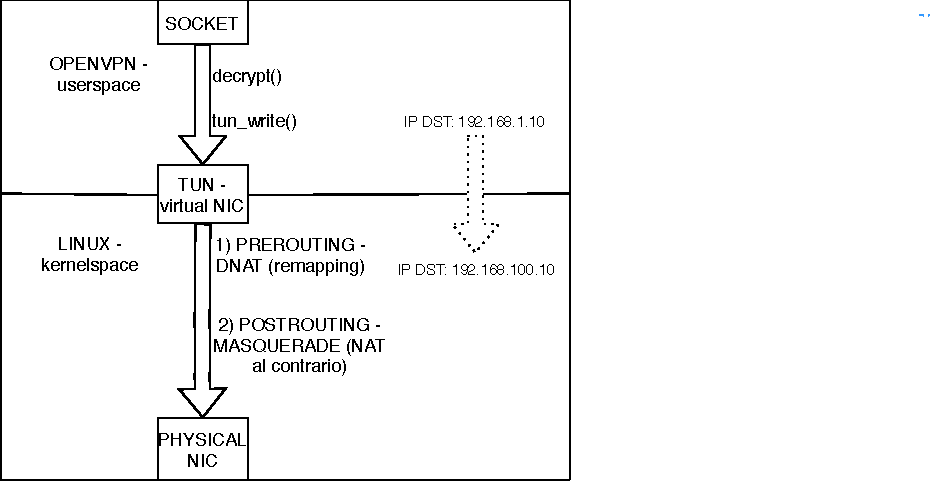
\includegraphics[scale=0.7]{img/ip_mapping_send}
		\label{fig:ip-mapping-send}
		\caption[IP Mapping: MoonCloud $\rightarrow$ Target]{
			IP Mapping: MoonCloud $\rightarrow$ Target. Si mostra un esempio di ciò che
			accade nel VPN client quando si riceve un pacchetto tramite la VPN.
			Per essere rigorosi occorre notare che una volta che OpenVPN invia qualcosa
			su un socket il controllo passa di nuovo al sistema operativo che scrive
			quindi il pacchetto sulla scheda di rete fisica, ma questo non è di interesse
		per il problema in questione.}
	\end{figure}
		
	\begin{figure}
		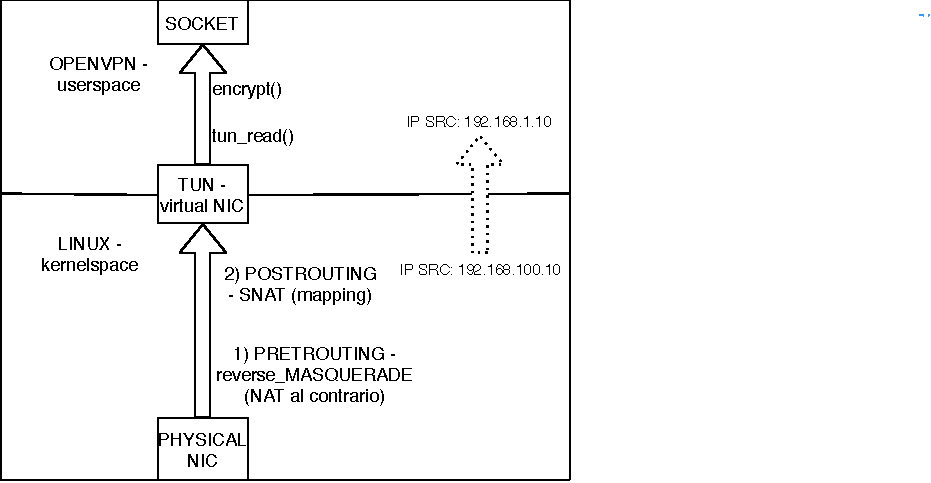
\includegraphics[scale=0.7]{img/ip_mapping_recv}
		\label{fig:ip-mapping-recv}
		\caption[IP Mapping: Target $\rightarrow$ MoonCloud]{
			IP Mapping: Target $\rightarrow$ MoonCloud. In questo caso si mostra
			cosa succede con i pacchetti in risposta a richieste provenienti
		da MoonCloud lungo la VPN.}
	\end{figure}
